\chapter{Phonologie}
\label{sec:phonologie}

\Voraussetzungen{Für das gesamte Kapitel sind gute Kenntnisse in der Definition und der Transkription der Standardaussprache unabdinglich (\EGBDRef{Phonetik}).
Die wichtigen Regularitäten des phonologischen Systems (segmental, silbenphonologisch und wortphonologisch) müssen bekannt sein (\EGBDRef{Phonologie}).
Die Begriffe \textit{Kern} und \textit{Peripherie} des Systems müssen geläufig sein (Teile von \EGBDRef{Grundlagen}), und die Grundzüge und Grundbegriffe der Flexion (\EGBDRef{Nominalflexion} und \EGBDRef{Verbalflexion}) und der Wortbildung (\EGBDRef{Wortbildung}) müssen bekannt sein.}

\section{Gegenstand der Phonologie}
\label{sec:phonologie:gegenstandderphonologie}

Die Phonologie beschreibt das \Mark[System, phonologisch]{phonologisches System} einer Sprache.
Mit \textit{System} ist einerseits gemeint, dass man von nicht bedeutungsrelevanten phonetischen Unterschieden einzelner Äußerungen abweicht.
Je nachdem, ob wir schneller oder langsamer sprechen, sind zum Beispiel die sogenannten \textit{langen Vokale} in Millisekunden gemessen unterschiedlich lang, und eine genaue phonetische Beschreibung von Äußerungen würde diese Längenunterschiede durchaus verzeichnen.
Trotzdem können Hörer in der Regel erkennen, ob die lange oder kurze Variante (lang wie in \textit{Hüte} [hyːtə] oder kurz wie in \textit{Hütte} [hʏtə]) artikuliert wurde, solange prinzipiell ein Längenunterschied gemacht wird.%
\footnote{Es kommt hinzu, dass die Länge und Kürze von Vokalen mit anderen Merkmalen zusammen auftritt und auch aus diesen erkennbar ist, welche Variante artikuliert wurde.
Im Deutschen ist besonders die \Mark{Vokalqualität} zu nennen, die auf besondere Weise mit Länge und Betonung interagiert.
Im gegebenen Beispiel sieht man das, weil [yː] und [ʏ] neben dem Längenunterschied auch an unterschiedlichen Orten artikuliert werden.
Siehe dazu die Diskussion zur \Mark{Gespanntheit} in \EGBDRef{Phonologie}.}
Andererseits ist das Lautsystem die Menge von Regularitäten, die auf Basis von möglichst redundanzfreien Repräsentationen von Wörtern und anderen Einheiten -- den \Mark{zugrundeliegenden Formen} -- alle konkreten phonetischen Artikulationen beschreibt.
Ein typisches Beispiel ist die \Mark{Silbifizierung}.
Ein Wort wie \textit{Tag} enthält im Nominativ Singular eine Silbe [taːk].
In allen Formen des Plurals wie \textit{Tage} [taː.gə] und im Genitiv Singular \textit{Tages} [taː.gəs] ist es jedoch zweisilbig, und die Silbengrenze (wie üblich mit dem Punkt .\ markiert) verläuft im Stamm des Wortes.
Die Silbengrenzen können also nicht mit dem Wort (einer irgendwie gearteten Grundform) im Lexikon abgelegt sein, sondern werden erst festgelegt, wenn die Wortform morphologisch vollständig ist.
Da die Silbengrenzen aber völlig regelhaft zugewiesen werden, braucht man eine Beschreibung des phonologischen Systems, um genau angeben zu können, wie die phonetischen Realisierungen von Wörtern und Wortformen systematisch zusammenhängen.

In diesem Kapitel wird das phonologische System in drei Teilbereiche eingeteilt.
In Abschnitt~\ref{sec:phonologie:analysenzursegmentalenphonologie} werden zunächst Phänomene betrachtet, die die Abfolge von Segmenten (den kleinsten Einheiten der Phonetik und Phonologie) betreffen.
Dabei geht es vor allem darum, wie sich Segmente verändern, wenn Sie in bestimmten Umgebungen auftreten.
In Abschnitt~\ref{sec:phonologie:analysenzursilbenphonologie} geht es um die Silbe.
Das Hauptproblem ist dabei die Festlegung der Silbengrenzen und damit automatisch auch der zulässigen Silbenstrukturen des Deutschen.
In Abschnitt~\ref{sec:phonologie:analysenzurwortphonologie} werden Übungen zu phonologischen Phänomenen auf Wortebene angeboten.
Im Zentrum stehen das phonologische und prosodische Wort und die Zuweisung des Akzents (also der Wortbetonung).
In diesem Abschnitt wird auch ausführlich darauf eingegangen, was der (morpho-)phonologische Kernwortschatz ist, und Kenntnisse in Flexion und Wortbildung sind daher unabdinglich.

\section{Analysen zur segmentalen Phonologie}
\label{sec:phonologie:analysenzursegmentalenphonologie}

\subsection{Strukturbedingungen der segmentalen Phonologie}
\label{sec:phonologie:strukturbedingungendersegmentalenphonologie}

In diesem Abschnitt werden zunächst die wichtigen \Mark{Strukturbedingungen} knapp zusammengefasst, die in \EGBDRef{Phonetik} (Abschnitt zu den Besonderheiten der Transkription), \EGBDRef{Phonologie} und \EGBDRef{Phonologische Schreibprinzipien} (Abschnitt zum Eszett und seinem phonologischen Korrelat) eingeführt wurden.
Alle diese Bedingungen führen dazu, dass zugrundeliegende Formen in konkreten Wortformen anders phonetisch realisiert werden als sie lexikalisch abgespeichert sind.
Zugrundeliegende Formen werden in /~/ geschrieben, phonetische Realisierungen in [~].
Das Wort \textit{Bank} ist zum Beispiel lexikalisch als /bank/ abgelegt, wird aber immer [baŋk] realisiert.
Welche Strukturbedingungen dazu führen, dass /n/ hier phonetisch zu [ŋ] wird, wird in den folgenden Absätzen beschrieben.
Diese Absätze haben wie in der Einleitung erläutert Wiederholungscharakter und sollten nach der Lektüre von EGBD vor Durchführung der nachfolgenden Übungen gelesen werden.

\paragraph*{Endrand"=Desonorisierung}

Im Deutschen kommen im Silbenendrand stimmlose und stimmhafte Konsonanten vor.
Der Liquid [l] im Einsilbler \textit{Ball} [bal] und der Nasal [n] im Einsilbler \textit{Bann} [ban] sind zum Beispiel stimmhaft.
Wenn aber sogenannte \textit{Obstruenten} (Plosive, Frikative und Affrikaten) im Silbenendrand stehen, müssen sie stimmlos sein.
Zugrundeliegende stimmhafte Obstruenten werden daher stimmlos.
Wenn in manchen Formen des Wortes das betreffende Segment allerdings im Anfangsrand steht, bleibt es stimmhaft, und die Annahme einer Strukturbedingung ist daher plausibel.

In (\ref{ex:endranddesonorisierung001})--(\ref{ex:endranddesonorisierung005}) werden einige Auswirkungen dieser Strukturbedingung illustriert.
Beispiel (\ref{ex:endranddesonorisierung005}) zeigt, dass auch innerhalb eines Wortes im Silbenendrand die Endrand"=Desonorisierung wirkt.

\begin{exe}
  \ex Bund \label{ex:endranddesonorisierung001}
  \begin{xlist}
    \ex /bʊnd/ $\Rightarrow$ [bʊnt]
    \ex /bʊndəs/ $\Rightarrow$ [bʊn.dəs]
  \end{xlist}
  \ex Steg \label{ex:endranddesonorisierung002}
  \begin{xlist}
    \ex /ʃteg/ $\Rightarrow$ [ʃteːk]
    \ex /ʃtegə/ $\Rightarrow$ [ʃteː.gə]
  \end{xlist}
  \ex Stab \label{ex:endranddesonorisierung003}
  \begin{xlist}
    \ex /ʃtab/ $\Rightarrow$ [ʃtaːb]
    \ex /ʃtabəs/ $\Rightarrow$ [ʃtaː.bəs]
  \end{xlist}
  \ex Los \label{ex:endranddesonorisierung004}
  \begin{xlist}
    \ex /loz/ $\Rightarrow$ [loːs]
    \ex /loze/ $\Rightarrow$ [loː.zə]
  \end{xlist}
  \ex lösen \label{ex:endranddesonorisierung005}
  \begin{xlist}
    \ex /løzən/ $\Rightarrow$ [løː.zən]
    \ex /løzlɪç/ $\Rightarrow$ [løːs.lɪç]
  \end{xlist}
\end{exe}

\paragraph*{/n/-Assimilation und [ŋ]}

Zugrundeliegendes /n/ wird innerhalb eines phonologischen Wortes an nachfolgende Velare im Artikulationsort angepasst.
Dies führt dazu, dass Wörter wie \textit{trinken} /tʁɪnkən/ als [tʁɪŋ.kən] realisiert werden.
Phonetisch kann es im Deutschen Wörter wie *[tʁɪn.kən] nicht geben.
Eingeschränkt und außerhalb des Standards findet diese Assimilation (Angleichung) auch bei folgenden Labialen statt.

Auf Basis dieser Strukturbedingung und einer Zusatzannahme ist es nicht erforderlich, das Segment [ŋ] in zugrundeliegenden Formen anzunehmen.
Wörter wie \textit{Angel} /angəl/ werden als [ʔaŋ̣əl] realisiert, weil das /n/ durch das folgende velare /g/  zu [ŋ] assimiliert wird.
Als Zusatzannahme muss davon ausgegangen werden, dass eine Abfolge *[ŋŋ] nicht möglich ist und ein [ŋ] gelöscht wird.
Im konkreten Beispiel ergibt sich dann ein Silbengelenk.

\paragraph*{Zugrundeliegendes /z/ und /s/}

Die grundlegende Verteilung von [z] und [s] ist relativ klar.
Im Silbenanfangsrand kommt nur [z] vor wie in \textit{Saft} [zaft], im Silbenendrand nur [s] wie in \textit{Tross} [tʁɔs].
Wäre dies ausnahmslos so, könnten wir zugrundeliegend prinzipiell immer /z/ annehmen (/zaft/, /tʁɔz/), und die Endrand-Desonorisierung würde dafür sorgen, dass es phonetisch keine Wörter wie *[tʁɔz] gibt.

Im Wortinneren an der Silbengrenze gibt es allerdings eine weitere Möglichkeit.
Nach gespannten (langen) Vokalen kann der Anfangsrand mit [s] besetzt sein wie in \textit{Muße} [muː.sə].%
\footnote{Nach ungespanntem Vokal läge im Kernwortschatz prinzipiell ein Silbengelenk vor, das grundsätzlich stimmlos ist, vgl.\ \textit{Blässe} [blɛṣə].}
Wie in \EGBDRef{Phonologie Schreibprinzipien} argumentiert wird, lässt sich diese Verteilung modellieren, wenn angenommen wird, dass in Wörtern wie \textit{Muße} zwei /z/ zugrundeliegen.
Eine Interaktion von verschiedenen, unabhängig motivierten Strukturbedingungen führt dann dazu, dass /muzzə/ als [muː.sə] realisiert wird.
Zugrundeliegend wird also für phonetisches [z] und [s] jeweils /z/ angenommen.

\paragraph*{Varianten von /ʁ/}

Der Liquid /ʁ/ hat im Deutschen besondere Realisierungen.
Im Anfangsrand wird er prinzipiell unverändert als [ʁ] ausgesprochen, im Endrand wird er vokalisiert.
Nach ungespannten Vokalen steht für /ʁ/ das Schwa [ə] und bildet mit dem Vokal einen Diphthong wie in \textit{Bar} /baʁ/ [ba͡ɐ], \textit{Tür} /tyʁ/ [ty͡ɐ], \textit{Rohr} /ʁoʁ/ [ʁo͡ɐ], \textit{mehr} /meʁ/ [me͡ɐ] oder \textit{Tier} /tiʁ/ [ti͡ɐ].
Nach gespannten Vokalen steht [ɐ] und bildet ebenfalls einen Diphthong wie in \textit{klirr} /klɪʁ/ [klɪ͡ə], \textit{knarr} /knăʁ/ [kna͡ə], \textit{Korb} /kɔʁb/ [kɔ͡əp] oder \textit{Berg} /bɛʁg/ [bɛ͡ək].
Die Verbindung von Schwa und /ʁ/ führt hingegen zu einer Silbe mit [ɐ] im Kern, zum Beispiel in \textit{unter} /ʊntəʁ/ [ʔʊn.tɐ], \textit{Fahrer} /faʁəʁ/ [faː.ʁɐ].

\paragraph*{Realisierungen von /ç/}

Die Frikative [ç] wie in \textit{Strich} [ʃtʁɪç] und [χ] wie in \textit{Fluch} [fluːχ] sind komplementär verteilt.
Vor nicht-vorderen Vokalen tritt [χ] auf, sonst immer [ç].
[χ] ist das uvulare Pendant zum palatalen [ç], und man kann daher davon ausgehen, dass vor nicht-vorderen Vokalen zugrundeliegendes /ç/ zu [χ] assimiliert wird.
Ein zugrundeliegendes /χ/ gibt es also nicht, und die zugrundeliegenden Formen zu den Beispielen sind /ʃtʁɪç/ und /fluːç/.

\paragraph*{/g/-Spirantisierung}

Im bundesdeutschen Standard wird /g/ nach /ɪ/ als [ç] realisiert, zum Beispiel in \textit{König} /kønɪg/ [køːnɪç].
Aufgrund anderer Formen dieses Worts wissen wir, dass hier /g/ zugrundeliegt, zum Beispiel \textit{Könige} /kønɪgə/ [kønɪgə].
In diesen Fällen geht [ç] also nicht auf /ç/ zurück.

\paragraph*{Einfügung des Glottalplosivs}

Diese Regularität wird aus technischen Gründen hier besprochen, könnte aber genauso gut in der Silben- oder Wortphonologie verortet werden.
In Silben, die entweder am Wortanfang oder am Fußanfang im Wortinneren stehen, und die keine Konsonanten im Anfangsrand haben, wird der glottale Plosiv [ʔ] eingefügt.
Ein Beispiel am Wortanfang wäre \textit{Ort} /ɔʁt/ [ʔɔ͡ət].
Im Wortinneren kommen neben dem Nicht-Kernwortschatz (\textit{sigmoid} /zɪgmoid/ [zɪk.mo.ˈʔiːt]) Worter mit Präfixen i.\,w.\,S.\ in Frage, zum Beispiel \textit{beenden} /bəɛ̆ndən/ [bə.ˈʔɛn.dən] oder \textit{anecken} /ănɛ̆kən/ [ˈʔan.ʔɛḳən]).

\paragraph*{Vokalqualität}

Die zugrundeliegenden Vokale des Deutschen können mit dem phonologischen Merkmal der \textit{Gespanntheit} unterschieden werden.
Abbildung~\ref{fig:gespanntheitbetonungundlaenge019} zeigt die Paare von gespannten und ungespannten Vokalen.
Es handelt sich bei der Gespanntheit nicht um ein vollständig phonetisch motivierbares Merkmal, da bei gespanntem /a/ und ungespanntem /ă/ und gespanntem /ɛ/ und ungespanntem /ɛ̆/ kein hörbarer Unterschied besteht.
Außerdem ist /ɛ̆/ die ungespannte Variante zu sowohl /e/ als auch /ɛ/.
Das Schwa /ə/ steht komplett außerhalb der Systeme der gespannten und ungespannten Vokale.

\begin{figure}[!htpb]
  \centering
  \begin{tikzpicture}[scale=3.5,baseline=default]
    \large
    \tikzset{
    vowel/.style={fill=white, anchor=mid, text depth=0ex, text height=1ex},
    vowelgespannt/.style={circle,fill=gray!30, anchor=mid, text depth=0ex, text height=1ex,minimum size=4ex},
    dot/.style={circle,fill=black,minimum size=0.4ex,inner sep=0pt,outer sep=-1pt},
    }

    \coordinate (hf) at (0,2); % high front
    \coordinate (hb) at (2,2); % high back
    \coordinate (lf) at (1,0); % low front
    \coordinate (lb) at (2,0); % low back
    \def\V(#1,#2){barycentric cs:hf={(3-#1)*(2-#2)},hb={(3-#1)*#2},lf={#1*(2-#2)},lb={#1*#2}}

    % Chart key (vorne -- hinten).
    \draw [{Latex[round]}-] (\V (-.25,0)) -- (\V (-.25,.5))  node [above left] {\footnotesize vorne};
    \draw [-{Latex[round]}] (\V (-.25,1.5)) -- (\V (-.25,2)) node [above left] {\footnotesize hinten};
    \path (\V (-.25,1)) node[above] {\footnotesize zentral};

    % Chart key (hoch--tief).
    \draw [{Latex[round]}-] (\V (0,-.25)) -- +(270:.5cm)  node [above right,rotate=90] (vokaltrapez1) {\footnotesize hoch};
    \draw [{Latex[round]}-] (\V (3,-2.5)) -- +(270:-.5cm) node [above left,rotate=90] (vokaltrapez2) {\footnotesize tief};
    \path (\V (1.5,-1)) node[above,rotate=90] {\footnotesize mittel};

    % Grid.
    \draw [gray,thick] (\V(0,0)) -- (\V(0,2));
    \draw [gray,thick] (\V(3,0)) -- (\V(3,2));
    \draw [gray,thick] (\V(0,0)) -- (\V(3,0));
    \draw [gray,thick] (\V(0,2)) -- (\V(3,2));

    \path (\V(0,0))      node[vowelgespannt] (i)   {i};
    \path (\V(0.25,0))   node[vowelgespannt] (y)   {y};
    \path (\V(0.4,0.5))  node[vowel]         (ii)  {ɪ};
    \path (\V(0.65,0.5)) node[vowel]         (yy)  {ʏ};
    \path (\V(1,0))      node[vowelgespannt] (e)   {e};
    \path (\V(1.25,0))   node[vowelgespannt] (oe)  {ø};
    \path (\V(2,0))      node[vowelgespannt] (ee)  {ɛ};
    \path (\V(1.4,0.7))  node[vowel]         (eee) {ɛ̆};
    \path (\V(1.65,0.7)) node[vowel]         (oee) {œ};
    \path (\V(3,1))      node[vowelgespannt] (a)   {a};
    \path (\V(2.5,1))    node[vowel]         (aa)  {ă};
    \path (\V (1,2))     node[vowelgespannt] (o)   {o};
    \path (\V (1.5,1.4)) node[vowel]         (oo)  {ɔ};
    \path (\V (0,2))     node[vowelgespannt] (u)   {u};
    \path (\V (0.5,1.5)) node[vowel]         (uu)  {ʊ};

    \draw (i)  -- (ii);
    \draw (y)  -- (yy);
    \draw (e)  -- (eee);
    \draw (oe) -- (oee);
    \draw (ee) -- (eee);
    \draw (a)  -- (aa);
    \draw (o)  -- (oo);
    \draw (u)  -- (uu);
  \end{tikzpicture}
  \caption[Phonologisches Vokaltrapez]{Phonologisches Vokaltrapez, gespannte Vokale grau hinterlegt}
  \label{fig:gespanntheitbetonungundlaenge019}
\end{figure}

Der Grund, die Zweiteilung nach Gespanntheit anzunehmen, liegt in der Interaktion von Gespanntheit, Betonung (Akzent) und Vokallänge im Kernwortschatz und Nicht-Kernwortschatz.
Im Kernwortschatz sind die gespannten Vokale immer betont und lang, im Nicht-Kernwortschatz sind sie lang, wenn sie betont sind und kurz, wenn sie nicht betont sind.
Die ungespannten Vokale verhalten sich im Kernwortschatz und Nicht-Kernwortschatz gleich.
Dort sind sie entweder betont oder unbetont, aber in jedem Fall immer kurz.
Schwa ist immer kurz und steht außerhalb der Systeme der gespannten und ungespannten, weil es niemals betont werden kann.

Zur Illustration folgen die Beispiele (\ref{ex:gespannt}) für gespannte Vokale im Kernwortschatz in der betonten langen Variante.
Beispiel (\ref{ex:gespanntsekdiphth}) zeigt, dass bei der Bildung sekundärer Diphthonge aus /ʁ/ der gespannte betonte Vokal nicht lang ist, weil es generell keine langen Vokale in Diphthongen gibt.
In (\ref{ex:ungespanntbetont}) werden Beispiele für betonte ungespannte Vokale im Kernwortschatz gezeigt.
Die entsprechenden unbetonten ungespannten Varianten werden in (\ref{ex:ungespanntunbetont}) bebeispielt.
Diese befinden sich typischerweise in Suffixen, und die gewählten Wörter sind daher keine Simplizia.
Sowohl in (\ref{ex:ungespanntbetont}) als auch (\ref{ex:ungespanntunbetont}) sind die ungespannten Vokale aber stets kurz.
Die Beispiele in (\ref{ex:nichtkernvokale}) illustrieren gespannte Vokale im Nicht-Kernwortschatz, die unbetont und daher nicht lang sind.
In (\ref{ex:gespanntfalschkurz}) werden nicht mögliche gespannte Vokale gezeigt, die betont und kurz sind.%
\footnote{Solche Vokale gibt es außerhalb des Standards zum Beispiel in regionalen Varianten des Ruhrgebiets und Westfalens.}
Solche Vokale gibt es weder im Kernwortschatz noch in Nicht-Kernwortschatz.%
\footnote{Das Zeichen ˈ steht vor der betonten Silbe, die in Simplizia des Kernwortschatzes immer die Erstsilbe ist.}

\begin{exe}
  \ex Kernwortschatz: gespannt → betont + lang (s.\ Erstsilbe) \label{ex:gespannt}
  \begin{xlist}
    \ex \textit{Ahne} /anə/ [ˈʔaː.nə]
    \ex \textit{Flug} /flug/ [ˈfluːk]
    \ex \textit{wenig} /venɪg/ [ˈveː.nɪç]
    \ex \textit{Tier} /tiʁ/ [ˈti͡ɐ] \label{ex:gespanntsekdiphth}
  \end{xlist}
  \ex Kernwortschatz: ungespannt + betont (s.\ Erstsilbe)\label{ex:ungespanntbetont}
  \begin{xlist}
    \ex \textit{Kanne} /kănə/ [ˈkaṇə]
    \ex \textit{Ruck} /ʁʊk/ [ˈʁʊk]
    \ex \textit{Ente} /ɛ̆ntə/ [ˈʔɛn.tə]
    \ex \textit{Birke} /bɪʁkə/ [ˈbɪ͡ə.kə]
  \end{xlist}
  \ex Kernwortschatz: ungespannt + unbetont (s.\ Suffixsilbe) \label{ex:ungespanntunbetont}
  \begin{xlist}
    \ex \textit{fügsam} /fygzăm/ [ˈfyːkzam]
    \ex \textit{Schenkung} /ʃɛnkʊng/ [ˈʃɛŋ.kʊŋ]
    \ex \textit{durchlässig} /dʊʁçlɛ̆zɪg/ [ˈdʊ͡əç.lɛṣɪç]
    \ex \textit{Neunziger} /nɔ͡œnt͡sɪgəʁ/ [ˈnɔ͡œn.t͡sɪ.gɐ]
  \end{xlist}
  \ex Nicht-Kernwortschatz: gespannt + unbetont → kurz (s.\ Erstsilben) \label{ex:nichtkernvokale}
  \begin{xlist}
    \ex \textit{Kanal} /kanal/ [ka.ˈnaːl]
    \ex \textit{Mutant} /mutant/ [mu.ˈtant]
    \ex \textit{Kerosin} /keʁozin/ [ke.ʁo.ˈziːn]
    \ex \textit{Figur} /figuʁ/ [fi.ˈgu͡ɐ]
  \end{xlist}
  \ex unmöglich: gespannt + betont + kurz \label{ex:gespanntfalschkurz}
  \begin{xlist}
    \ex /bunt/ *[ˈbunt]
    \ex /kin/ *[ˈkin]
  \end{xlist}
  \ex unmöglich: gespannt + unbetont + lang (s.\ Endsilbe) \label{ex:gespanntfalschlang}
  \begin{xlist}
    \ex /metyl/ *[ˈme.tyːl]
    \ex /byʁo/ *[ˈby.ʁoː]
  \end{xlist}
\end{exe}

Als Folge dieser Regularitäten wird in zugrundeliegenden Formen die Länge nicht spezifiziert.
Sie kann aus der Gespanntheit und der Betonung abgeleitet werden.
Eigentlich müsste aber die Betonung (zumindest im Nicht-Kernwortschatz) lexikalisch -- also in den zugrundeliegenden Formen -- spezifiziert werden.%
\footnote{Dies müsste sie ohnehin, denn die Betonung in Nicht-Kernwortschatz-Wörtern mit Stämmen, die nicht auf der ersten Silbe betont sind, wie \textit{Kanal} ist prinzipiell nicht vorhersagbar.
Das Gleiche gilt für Erbwörter im Nicht-Kernwortschatz wie \textit{warum}, \textit{vielleicht}, \textit{Bovist} usw.}
Da es keine Silben in den zugrundeliegenden Formen gibt, kann der Akzent nur für die Vokale spezifiziert werden.
Wir lassen diese Akzentnotation hier aus Gründen der Übersichtlichkeit weg, aber präzise müsste man die zugrundeliegenden Formen in (\ref{ex:nichtkernvokale}) als /kanál/, /mutánt/, /keʁozín/ und /figúʁ/ notieren.

\subsection{Übungen}


\vspace{2\baselineskip}
\Uebung{Zugrundeliegende Formen}{%
Wir arbeiten in diesem Kapitel weiter mit dem Text~\ref{text:weltraum} (S.~\pageref{text:weltraum}).
Geben Sie die zugrundeliegenden Formen zu den phonetischen Realisierungen an, die Sie in Kapitel~\ref{sec:phonetik} erstellt haben.
}

\paragraph*{Teillösung}

Hier wird die phonetische Transkription mit den zugrundeliegenden Formen interlinear gegeben.

\begin{exe}
  \ex \gll de͡ɐ vɛltʁa͡ɔm bət͡sa͡ɛçnət deːn ʁa͡ɔm t͡svɪʃən hɪməlskœ͡əpɐn\\
  deʁ vɛ̆ltʁa͡ɔm bət͡sa͡ɛçnət den ʁa͡ɔm t͡svɪʃən hɪməlzkœʁpəʁn\\
  \ex \gll diː atmosfɛːrən vɔn fɛstən ʊnt gaːsfœ͡əmɪgən hɪməlskœ͡əpɐn viː ʃtɛ͡ənən ʔʊnt planeːtən haːbən ka͡ɛnə fɛstə gʁɛnt͡sə naːχ ʔoːbən zɔndɐn vɛ͡ədən mɪt t͡suːneːməndəm ʔapʃtant t͡sʊm hɪməlskœ͡əpɐ almɛːlɪç ʔɪmɐ dʏnɐ\\
  di ătmozfɛrən vɔn fɛ̆ztən ʔʊnt gazfœʁmɪgən hɪməlzkœʁpəʁn vi ʃtɛ̆ʁnən ʊnt plănetən habən ka͡ɛnə fɛ̆ztə gʁɛ̆nt͡sə naç obən zɔndəʁn vɛ̆ʁdən mɪt t͡suneməndəm ăpʃtănd t͡sʊm hɪməlzkœʁpəʁ ălmɛlɪç ɪməʁ dʏnəʁ\\
  \ex \gll ʔap ʔa͡ɛnɐ bəʃtɪmtən høːə ʃpʁɪçt man fɔm bəgɪn dəs vɛltʁa͡ɔms\\
  ăp a͡ɛnəʁ bəʃtɪmtən høə ʃpʁɪçt măn fɔm bəgɪn dəz vɛ̆ltʁa͡ɔmz\\
  \ex \gll ʔɪm vɛltʁa͡ɔm hɛ͡əʃt ʔa͡ɛn hoːχvaːkuʔʊm mɪt niːdʁɪgɐ ta͡ɛlçəndɪçtə\\
  ɪm vɛ̆ltʁa͡ɔm hɛʁʃt a͡ɛn hoçvakuʊm mɪt nidʁɪgəʁ ta͡ɛlçəndɪçtə\\
  \ex \gll ʔe͡ɐ ʔɪst ʔaːbɐ ka͡ɛn leːrɐ ʁa͡ɔm zɔndɐn ʔɛnthɛlt gaːzə kɔsmɪʃən ʃta͡ɔp ʔʊnt ʔɛləmɛnta͡ɐta͡ɛlçən nɔ͡œtʁiːnos kɔsmɪʃə ʃtʁaːlʊŋ pa͡ətikəl ʔa͡ɔsɐdeːm ʔelɛktʁɪʃə ʔʊnt magneːtɪʃə fɛldɐ gʁavitat͡sioːnsfɛldɐ ʔʊnt ʔelɛktʁomagneːtɪʃə vɛlən fotoːnən\\
  eʁ ɪzt abəʁ ka͡ɛn lerəʁ ʁa͡ɔm zɔndəʁn ɛ̆nthɛ̆lt gazə kɔzmɪʃən ʃta͡ɔb ʊnt ɛ̆ləmɛ̆ntaʁta͡ɛlçən nɔ͡œtʁinoz kɔzmɪʃə ʃtʁalʊng paʁtikəl a͡ɔzzəʁdem elɛ̆ktʁɪʃə ʊnt măgnetɪʃə fɛ̆ldəʁ gʁăvităt͡sionsfɛ̆ldɐ ʊnt elɛktʁomagnetɪʃə vɛ̆lən fotonən\\
  \ex \gll das fast fɔlʃtɛndɪgə vaːkuʔʊm ʔɪm vɛltʁa͡ɔm maχt ʔiːn ʔa͡ɔsɐʔɔ͡ədəntlɪç dʊ͡əçzɪçtɪç ʔʊnt ʔɛ͡əla͡ɔpt diː bəʔoːbaχtʊŋ ʔɛkstʁeːm ʔɛntfɛ͡əntɐ ʔɔpjɛktə ʔɛtvaː ʔandəʁɐ galaksiːən\\
  dăz făst fɔlʃtɛ̆ndɪgə vakuʊm ɪm vɛ̆ltʁa͡ɔm măçt in a͡ɔzzəʁʔɔʁdəntlɪç dʊʁçzɪçtɪg ʊnt ɛ̆ʁla͡ɔbt di bəobăçtʊng ɛ̆kztʁem ɛ̆ntfɛ̆ʁntəʁ ɔpjɛ̆ktə ɛ̆tva ăndəʁəʁ gălăkziən\\
  \ex \gll jedɔχ kœnən neːbəl ʔa͡ɔs ʔɪntɐstɛlaːʁɐ mateːʁiə diː zɪçt ʔa͡ɔf dahɪntɐliːgəndə ʔɔpjɛktə ʔa͡ɔχ ʃta͡ək bəhɪndɐn\\
  jedɔχ kœnən nebəl a͡ɔz ɪntəʁstɛ̆laʁəʁ măteʁiə di zɪçt a͡ɔf dăhɪntəʁligəndə ɔpjɛ̆ktə a͡ɔç ʃtăʁk bəhɪndəʁn\\
\end{exe}

Beim Ermitteln der zugrundeliegenden Formen auf Basis der phonetischen Transkription ist zu beachten, dass für jedes [ɛ] und [a] entschieden werden muss, ob sie der ungespannten Variante wie in /măn/ oder der gespannten Variante wie in /abəʁ/ entsprechen.
Im Kernwortschatz sind sie lang und betont (und dann immer gespannt, also /a/ oder /ɛ/) oder kurz und unbetont (und dann ungespannt, also /ă/ bzw.\ /ɛ̆/).
Wenn sie im Nicht-Kernwortschatz unbetont sind, ist diese Frage wegen der gleichen Artikulation der gespannten und ungespannten Variante nicht zu entscheiden, und hier wurde durchgehend die ungespannte Variante angenommen, zum Beispiel in /elɛ̆ktʁɪʃə/ oder /gălăksiən/.


\Uebung{Strukturbedingungen (segmental)}{%
Finden Sie auf Basis der zugrundeliegenden Formen und der phonetischen Transkription möglichst viele Beispiele für die Strukturbedingungen aus Abschnitt~\ref{sec:phonologie:strukturbedingungendersegmentalenphonologie} mit Ausnahme der Effekte der Gespanntheit.
Konkret sind dies:

\begin{enumerate}
  \item Endrand"=Desonorisierung inkl.\ /z/ $\Rightarrow$ [s]
  \item /n/-Assimilation
  \item {}[ŋ]-Bildung
  \item Fälle von zugrundeliegendem /zz/
  \item /ʁ/ als [ə] im sekundären Diphthong
  \item /ʁ/ als [ɐ] im sekundären Diphthong
  \item {}[ɐ] als Produkt von /əʁ/
  \item Realisierungen von /ç/ inkl.\ der Angabe des Auslösers, falls [χ] realisiert wird
  \item spirantisiertes /g/
  \item eingefügte Glottalplosive [ʔ]
\end{enumerate}
}

\paragraph*{Teillösung}

Die Lösung bezieht sich nur auf den oben transkribierten Teil des Texts.
Wiederholungen und mehrere Formen desselben Wortes werden hier nicht aufgelistet.

\vspace{1\baselineskip}
\begin{longtable}[l]{p{0.1mm}lcll}
  \multicolumn{5}{l}{\textbf{Endrand"=Desonorisierung}}                                            \\
    & /hɪməlzkœʁpəʁn/    & $\Rightarrow$ & [hɪməlskœ͡əpɐn]      &                                   \\
    & /fɛ̆ztən/           & $\Rightarrow$ & [fɛstən]            &                                   \\
    & /gazfœʁmɪgən/      & $\Rightarrow$ & [gaːsfœ͡əmɪgən]      &                                   \\
    & /ăpʃtănd/          & $\Rightarrow$ & [ʔapʃtant]          & wegen /ăp/ s.\ Anmerkungen        \\
    & /dəz/              & $\Rightarrow$ & [dəs]               &                                   \\
    & /vɛ̆ltʁa͡ɔmz/        & $\Rightarrow$ & [vɛltʁa͡ɔms]         &                                   \\
    & /ɪzt/              & $\Rightarrow$ & [ʔɪst]              &                                   \\
    & /kɔzmɪʃən/         & $\Rightarrow$ & [kɔsmɪʃən]          &                                   \\
    & /ʃta͡ɔb/            & $\Rightarrow$ & [ʃta͡ɔp]             &                                   \\
    & /dăz/              & $\Rightarrow$ & [das]               &                                   \\
    & /ɛ̆kztʁem/          & $\Rightarrow$ & [ʔɛkstʁeːm]         &                                   \\
    & /gălăkziən/        & $\Rightarrow$ & [gălăkziən]         &                                   \\
    & /a͡ɔz/              & $\Rightarrow$ & [ʔa͡ɔs]              &                                   \\
  \multicolumn{5}{l}{ }                                                                            \\
  \multicolumn{5}{l}{\textbf{/n/-Assimilation}}                                                    \\
    & \multicolumn{4}{l}{kommt im Textausschnitt nicht vor}                                        \\
  \multicolumn{5}{l}{ }                                                                            \\
  \multicolumn{5}{l}{\textbf{/ng/ $\Rightarrow$ [ŋ]}}                                              \\
    & /ʃtʁalʊng/         & $\Rightarrow$ & [ʃtʁaːlʊŋ]          &                                   \\
    & /bəobăçtʊng/       & $\Rightarrow$ & [bəʔoːbaχtʊŋ]       &                                   \\
  \multicolumn{5}{l}{ }                                                                            \\
  \multicolumn{5}{l}{\textbf{/zz/ $\Rightarrow$ [s]}}                                              \\
    & /a͡ɔzzəʁdem/        & $\Rightarrow$ & [ʔa͡ɔsɐdeːm]         &                                   \\
    & /a͡ɔzzəʁʔɔʁdəntlɪç/ & $\Rightarrow$ & [ʔa͡ɔsɐʔɔ͡ədəntlɪç]   &                                   \\
  \multicolumn{5}{l}{ }                                                                            \\
  \multicolumn{5}{l}{\textbf{/ʁ/ $\Rightarrow$ [ə]}}                                               \\
    & /hɪməlzkœʁpəʁn/    & $\Rightarrow$ & [hɪməlskœ͡əpɐn]      &                                   \\
    & /gazfœʁmɪgən/      & $\Rightarrow$ & [gaːsfœ͡əmɪgən]      &                                   \\
    & /ʃtɛ̆ʁnən/          & $\Rightarrow$ & [ʃtɛ͡ənən]           &                                   \\
    & /vɛ̆ʁdən/           & $\Rightarrow$ & [vɛ͡ədən]            &                                   \\
    & /hɛʁʃt/            & $\Rightarrow$ & [hɛ͡əʃt]             &                                   \\
    & /paʁtikəl/         & $\Rightarrow$ & [pa͡ətikəl]          &                                   \\
    & /a͡ɔzzəʁʔɔʁdəntlɪç/ & $\Rightarrow$ & [ʔa͡ɔsɐʔɔ͡ədəntlɪç]   &                                   \\
    & /dʊʁçzɪçtɪg/       & $\Rightarrow$ & [dʊ͡əçzɪçtɪç]        &                                   \\
    & /ɛ̆ʁla͡ɔbt/          & $\Rightarrow$ & [ʔɛ͡əla͡ɔpt]          &                                   \\
    & /ɛ̆ntfɛ̆ʁntəʁ/       & $\Rightarrow$ & [ʔɛntfɛ͡əntɐ]        &                                   \\
    & /ʃtăʁk/            & $\Rightarrow$ & [ʃta͡ək]             &                                   \\
  \multicolumn{5}{l}{ }                                                                            \\
  \multicolumn{5}{l}{\textbf{/ʁ/ $\Rightarrow$ [ɐ]}}                                               \\
    & /deʁ/              & $\Rightarrow$ & [de͡ɐ]               &                                   \\
    & /eʁ/               & $\Rightarrow$ & [ʔe͡ɐ]               &                                   \\
    & /ɛ̆ləmɛ̆ntaʁta͡ɛlçən/ & $\Rightarrow$ & [ʔɛləmɛnta͡ɐta͡ɛlçən] &                                   \\
  \multicolumn{5}{l}{ }                                                                            \\
  \multicolumn{5}{l}{\textbf{/əʁ/ $\Rightarrow$ [ɐ]}}                                              \\
    & /hɪməlzkœʁpəʁn/    & $\Rightarrow$ & [hɪməlskœ͡əpɐn]      &                                   \\
    & /zɔndəʁn/          & $\Rightarrow$ & [zɔndɐn]            &                                   \\
    & /ɪməʁ/             & $\Rightarrow$ & [ʔɪmɐ]              &                                   \\
    & /dʏnəʁ/            & $\Rightarrow$ & [dʏnɐ]              &                                   \\
    & /a͡ɛnəʁ/            & $\Rightarrow$ & [ʔa͡ɛnɐ]             &                                   \\
    & /nidʁɪgəʁ/         & $\Rightarrow$ & [niːdʁɪgɐ]          &                                   \\
    & /abəʁ/             & $\Rightarrow$ & [ʔaːbɐ]             &                                   \\
    & /lerəʁ/            & $\Rightarrow$ & [leːrɐ]             &                                   \\
    & /a͡ɔzzəʁdem/        & $\Rightarrow$ & [ʔa͡ɔsɐdeːm]         &                                   \\
    & /fɛ̆ldəʁ/           & $\Rightarrow$ & [fɛldɐ]             &                                   \\
    & /a͡ɔzzəʁʔɔʁdəntlɪç/ & $\Rightarrow$ & [ʔa͡ɔsɐʔɔ͡ədəntlɪç]   &                                   \\
    & /ɛ̆ntfɛ̆ʁntəʁ/       & $\Rightarrow$ & [ʔɛntfɛ͡əntɐ]        &                                   \\
    & /ăndəʁəʁ/          & $\Rightarrow$ & [ʔandəʁɐ]           &                                   \\
    & /ɪntəʁstɛ̆laʁəʁ/    & $\Rightarrow$ & [ʔɪntɐstɛlaːʁɐ]     &                                   \\
    & /dăhɪntəʁligəndə / & $\Rightarrow$ & [dahɪntɐliːgəndə]   &                                   \\
    & /bəhɪndəʁn/        & $\Rightarrow$ & [bəhɪndɐn]          &                                   \\
  \multicolumn{5}{l}{ }                                                                            \\
  \multicolumn{5}{l}{\textbf{Realisierungen von /ç/}}                                              \\
    & /bət͡sa͡ɛçnət/       & $\Rightarrow$ & [bət͡sa͡ɛçnət]        &                                   \\
    & /naç/              & $\Rightarrow$ & [naːχ]              & /a/ (zentral) geht voraus         \\
    & /ălmɛlɪç/          & $\Rightarrow$ & [almɛːlɪç]          &                                   \\
    & /ʃpʁɪçt/           & $\Rightarrow$ & [ʃpʁɪçt]            &                                   \\
    & /hoçvakuʊm/        & $\Rightarrow$ & [hoːχvaːkuʔʊm]      & /o/ (hinten) geht voraus          \\
    & /ta͡ɛlçəndɪçtə/     & $\Rightarrow$ & [ta͡ɛlçəndɪçtə]      &                                   \\
    & /măçt/             & $\Rightarrow$ & [maχt]              & /a/ (zentral) geht voraus         \\
    & /a͡ɔzzəʁʔɔʁdəntlɪç/ & $\Rightarrow$ & [ʔa͡ɔsɐʔɔ͡ədəntlɪç]   &                                   \\
    & /dʊʁçzɪçtɪg/       & $\Rightarrow$ & [dʊ͡əçzɪçtɪç]        &                                   \\
    & /bəobăçtʊng/       & $\Rightarrow$ & [bəʔoːbaχtʊŋ]       & /a/ (zentral) geht voraus         \\
    & /jedɔχ/            & $\Rightarrow$ & [jedɔχ]             & /o/ (hinten) geht voraus          \\
    & /zɪçt/             & $\Rightarrow$ & [zɪçt]              &                                   \\
    & /a͡ɔç/              & $\Rightarrow$ & [ʔa͡ɔχ]              & /a͡ɔ/ (hinten) geht voraus         \\
  \multicolumn{5}{l}{ }                                                                            \\
  \multicolumn{5}{l}{\textbf{/g/-Spirantisierung}}                                                 \\
    & /dʊʁçzɪçtɪg/       & $\Rightarrow$ & [dʊ͡əçzɪçtɪç]        &                                   \\
  \multicolumn{5}{l}{ }                                                                            \\
  \multicolumn{5}{l}{\textbf{eingefügte Glottalplosive}}                                           \\
    & /ʊnd/              & $\Rightarrow$ & [ʔʊnt]              &                                   \\
    & /obən/             & $\Rightarrow$ & [ʔoːbən]            &                                   \\
    & /ăpʃtănd/          & $\Rightarrow$ & [ʔapʃtant]          &                                   \\
    & /ɪməʁ/             & $\Rightarrow$ & [ʔɪmɐ]              &                                   \\
    & /ăp/               & $\Rightarrow$ & [ʔap]               &                                   \\
    & /a͡ɛnəʁ/            & $\Rightarrow$ & [ʔa͡ɛnɐ]             &                                   \\
    & /ɪm/               & $\Rightarrow$ & [ʔɪm]               &                                   \\
    & /a͡ɛn/              & $\Rightarrow$ & [ʔa͡ɛn]              &                                   \\
    & /hoçvakuʊm/        & $\Rightarrow$ & [hoːχvaːkuʔʊm]      & im Wortinnern                     \\
    & /eʁ/               & $\Rightarrow$ & [ʔe͡ɐ]               &                                   \\
    & /ɪzt/              & $\Rightarrow$ & [ʔɪst]              &                                   \\
    & /abəʁ/             & $\Rightarrow$ & [ʔaːbɐ]             &                                   \\
    & /ɛ̆nthɛ̆lt/          & $\Rightarrow$ & [ʔɛnthɛlt]          &                                   \\
    & /ɛ̆ləmɛ̆ntaʁta͡ɛlçən/ & $\Rightarrow$ & [ʔɛləmɛnta͡ɐta͡ɛlçən] &                                   \\
    & /a͡ɔzəʁdem/         & $\Rightarrow$ & [ʔa͡ɔsɐdeːm]         &                                   \\
    & /elɛ̆ktʁɪʃə/        & $\Rightarrow$ & [ʔelɛktʁɪʃə]        &                                   \\
    & /in/               & $\Rightarrow$ & [ʔiːn]              &                                   \\
    & /a͡ɔzzəʁʔɔʁdəntlɪç/ & $\Rightarrow$ & [ʔa͡ɔsɐʔɔ͡ədəntlɪç]   &                                   \\
    & /ɛ̆ʁla͡ɔbt/          & $\Rightarrow$ & [ʔɛ͡əla͡ɔpt]          &                                   \\
    & /bəobăçtʊng/       & $\Rightarrow$ & [bəʔoːbaχtʊŋ]       & im Wortinnern nach Präfix         \\
    & /ɛ̆kztʁem/          & $\Rightarrow$ & [ʔɛkstʁeːm]         &                                   \\
    & /ɛ̆ntfɛ̆ʁntəʁ/       & $\Rightarrow$ & [ʔɛntfɛ͡əntɐ]        &                                   \\
    & /ɔpjɛ̆ktə/          & $\Rightarrow$ & [ʔɔpjɛktə]          &                                   \\
    & /ɛ̆tva/             & $\Rightarrow$ & [ʔɛtvaː]            &                                   \\
    & /ăndəʁəʁ/          & $\Rightarrow$ & [ʔandəʁɐ]           &                                   \\
    & /a͡ɔz/              & $\Rightarrow$ & [ʔa͡ɔs]              &                                   \\
    & /ɪntəʁstɛ̆laʁəʁ/    & $\Rightarrow$ & [ʔɪntɐstɛlaːʁɐ]     &                                   \\
    & /a͡ɔf/              & $\Rightarrow$ & [ʔa͡ɔf]              &                                   \\
    & /a͡ɔç/              & $\Rightarrow$ & [ʔa͡ɔχ]              &                                   \\
\end{longtable}

\paragraph*{Anmerkungen}

In Wörtern wie \textit{und} oder dem Präfix \textit{ab-} wie \textit{Abstand} /ăpʃtănd/ [ʔapʃtant] liegt trotz der Schreibung mit dem Zeichen für den jeweiligen stimmhaften Konsonanten keine Endrand-Desonorisierung vor, da diese Wörter bzw.\ Affixe keine anderen Formen haben, in denen der stimmhafte Plosiv realisiert wird.

\Uebung{Gespanntheit}{%
Finden Sie für jede der Typen von Vokalen, die oben zum Thema Gespanntheit besprochen wurden, möglichst viele Beispiele.
Im Einzelnen:

\begin{enumerate}
  \item gespannte Vokale, die betont und lang sind
  \item gespannte Vokale, die unbetont und kurz sind
  \item ungespannte Vokale, die unbetont sind
  \item ungespannte Vokale, die betont sind
\end{enumerate}
}

Klassifizieren Sie die Wörter auf Basis der Vokalqualitäten als Kernwortschatz oder Nicht-Kernwortschatz.

\paragraph*{Teillösung}

Der Akzent (einschließlich Nebenakzent) wird hier zur Verdeutlichung verzeichnet, auch wenn die Silbenstruktur ansonsten noch nicht analysiert wurde.
Falls mehrere identische Vokale im Wort vorkommen, werden diese durchnumeriert mit Indizes, also [a]\Sub{1}, [a]\Sub{2} usw.

\begin{longtable}[l]{p{0.1mm}lll}
  \multicolumn{3}{l}{\textbf{Gespannte Vokale, die betont und lang sind}}    \\
  & [ˈdeːn]                  & [eː]                                          \\
  & [ˈdiː]                   & [iː]                                          \\
  & [ˈviː]                   & [iː]                                          \\
  & [plaˈneːtən]             & [eː]                                          \\
  & [ˈhaːbən]                & [aː]                                          \\
  & [ˈnaːχ]                  & [aː]                                          \\
  & [ˈʔoːbən]                & [oː]                                          \\
  & [ˈt͡suːˌneːməndəm]        & [uː] [eː]                                     \\
  & [alˈmɛːlɪç]              & [ɛː]                                          \\
  & [ˈhøːə]                  & [øː]                                          \\
  & [ˈhoːχˌvaːkuʔʊm]         & [oː] [aː]                                     \\
  & [ˈniːdʁɪgɐ]              & [iː]                                          \\
  & [ˈʔaːbɐ]                 & [aː]                                          \\
  & [ˈleːrɐ]                 & [eː]                                          \\
  & [ˈgaːzə]                 & [aː]                                          \\
  & [nɔ͡œˈtʁiːnos]            & [iː]                                          \\
  & [ˈʃtʁaːlʊŋ]              & [aː]                                          \\
  & [ˈʔa͡ɔsɐˌdeːm]            & [eː]                                          \\
  & [maˈgneːtɪʃə]            & [eː]                                          \\
  & [gʁavitaˈt͡sioːnsˌfɛldɐ]  & [oː]                                          \\
  & [foˈtoːnən]              & [oː]                                          \\
  & [ˈvaːkuʔʊm]              & [aː]                                          \\
  & [ˈʔiːn]                  & [iː]                                          \\
  & [ˈdiː]                   & [iː]                                          \\
  & [bəˈʔoːbaχtʊŋ]           & [oː]                                          \\
  & [ʔɛksˈtʁeːm]             & [eː]                                          \\
  & [galakˈsiːən]            & [iː]                                          \\
  & [ˈneːbəl]                & [eː]                                          \\
  & [ʔɪntɐstɛˈlaːʁɐ]         & [aː]                                          \\
  & [maˈteːʁiə]              & [eː]                                          \\
  & [daˈhɪntɐˌliːgəndə]      & [iː]                                          \\
  \multicolumn{3}{l}{ }                                                      \\
  \multicolumn{3}{l}{\textbf{Gespannte Vokale, die unbetont und kurz sind}}  \\
  & [atmosˈfɛːrən]            & [o]                                          \\
  & [ˈhoːχvaːkuˌʔʊm]         & [u]                                           \\
  & [nɔ͡œˈtʁiːnos]            & [o]                                           \\
  & [gʁavitaˈt͡sioːnsˌfɛldɐ]  & [i] [i]                                       \\
  & [ʔeˈlɛktʁomaˌgneːtɪʃə]   & [e] [o]                                       \\
  & [foˈtoːnən]              & [o]                                           \\
  & [maˈteːʁiə]              & [i]                                           \\
  \multicolumn{3}{l}{ }                                                      \\
  \multicolumn{3}{l}{\textbf{Ungespannte Vokale, die unbetont sind}}         \\
  & [atmosˈfɛrən]            & [a]                                           \\
  & [ˈgasˌfœ͡əmɪgən]          & [ɪ]                                           \\
  & [plaˈneːtən]             & [a]                                           \\
  & [ˈʔapʃtant]              & [a]\Sub{2}                                    \\
  & [ˈniːdʁɪgɐ]              & [ɪ]                                           \\
  & [ʔɛntˈhɛlt]              & [ɛ]\Sub{1}                                    \\
  & [ˈkɔsmɪʃən]              & [ɪ]                                           \\
  & [ʔɛləmɛnˈta͡ɐˌta͡ɛlçən]    & [ɛ]\Sub{1} [ɛ]\Sub{2}                         \\
  & [ˈkɔsmɪʃə]               & [ɪ]                                           \\
  & [ˈʃtʁaːlʊŋ]              & [ʊ]                                           \\
  & [ʔɛˈlɛktʁɪʃə]            & [ɛ]\Sub{1} [ɪ]                                \\
  & [maˈgneːtɪʃə]            & [a] [ɪ]                                       \\
  & [gʁavitaˈt͡sioːnsˌfɛldɐ]  & [a]\Sub{1} [a]\Sub{2} [ɛ]                     \\
  & [ˈfɔlˌʃtɛndɪgə]          & [ɛ] [ɪ]                                       \\
  & [ˌʔa͡ɔsɐˈʔɔ͡ədəntlɪç]      & [ɪ]                                           \\
  & [ˈdʊ͡əçˌzɪçtɪç]           & [ɪ]\Sub{2}                                    \\
  & [bəˈʔoːbaχtʊŋ]           & [a] [ʊ]                                       \\
  & [ʔɛksˈtʁeːm]             & [ɛ]                                           \\
  & [ʔɛntˈfɛ͡əntɐ]            & [ɛ]                                           \\
  & [ʔɔpˈjɛktə]              & [ɔ]                                           \\
  & [galakˈsiːən]            & [a]\Sub{1} [a]\Sub{2}                         \\
  & [ˌʔɪntɐstɛˈlaːʁɐ]        & [ɛ]                                           \\
  & [maˈteːʁiə]              & [a]                                           \\
  & [daˈhɪntɐˌliːgəndə]      & [a]                                           \\
  \multicolumn{3}{l}{ }                                                      \\
  \multicolumn{3}{l}{\textbf{Ungespannte Vokale, die betont sind}}           \\
  & [ˈvɛltˌʁa͡ɔm]             & [ɛ]                                           \\
  & [ˈt͡svɪʃən]               & [ɪ]                                           \\
  & [ˈhɪməlsˌkœ͡əpɐn]         & [ɪ]                                           \\
  & [ˈvɔn]                   & [ɔ]                                           \\
  & [ˈfɛstən]                & [ɛ]                                           \\
  & [ˈʔʊnt]                  & [ʊ]                                           \\
  & [ˈgʁɛnt͡sə]               & [ɛ]                                           \\
  & [ˈzɔndɐn]                & [ɔ]                                           \\
  & [ˈmɪt]                   & [ɪ]                                           \\
  & [ˈʔapʃtant]              & [a]\Sub{1}                                    \\
  & [ˈt͡sʊm]                  & [ʊ]                                           \\
  & [alˈmɛːlɪç]              & [ɛ]                                           \\
  & [ˈʔɪmɐ]                  & [ɪ]                                           \\
  & [ˈdʏnɐ]                  & [ʏ]                                           \\
  & [ˈʔap]                   & [a]                                           \\
  & [bəˈʃtɪmtən]             & [ɪ]                                           \\
  & [ˈʃpʁɪçt]                & [ɪ]                                           \\
  & [ˈman]                   & [a]                                           \\
  & [ˈfɔm]                   & [ɔ]                                           \\
  & [bəˈgɪn]                 & [ɪ]                                           \\
  & [ˈʔɪm]                   & [ɪ]                                           \\
  & [ˈhoːχˌvaːkuʔˌʊm]        & [ʊ]                                           \\
  & [ˈta͡ɛlçənˌdɪçtə]         & [ɪ]                                           \\
  & [ʔɛntˈhɛlt]              & [ɛ]\Sub{2}                                    \\
  & [ˈkɔsmɪʃən]              & [ɔ]                                           \\
  & [ʔɛˈlɛktʁɪʃə]            & [ɛ]\Sub{2}                                    \\
  & [ˈfɛldɐ]                 & [ɛ]                                           \\
  & [gʁavitaˈt͡sioːnsˌfɛldɐ]  & [ɛ]                                           \\
  & [ˈvɛlən]                 & [ɛ]                                           \\
  & [ˈdas]                   & [a]                                           \\
  & [ˈfast]                  & [a]                                           \\
  & [ˈfɔlˌʃtɛndɪgə]          & [ɔ] [ɛ]                                       \\
  & [ˈvaːkuʔˌʊm]             & [a]                                           \\
  & [ˈmaχt]                  & [a]                                           \\
  & [ˈdʊ͡əçˌzɪçtɪç]           & [ɪ]\Sub{1}                                    \\
  & [ʔɔpˈjɛktə]              & [ɛ]                                           \\
  & [ˈʔɛtvaː]                & [ɛ]                                           \\
  & [ˈʔandəʁɐ]               & [a]                                           \\
  & [jeˈdɔχ]                 & [ɔ]                                           \\
  & [ˈkœnən]                 & [œ]                                           \\
  & [ˌʔɪntɐstɛˈlaːʁɐ]        & [ɪ]                                           \\
  & [ˈzɪçt]                  & [ɪ]                                           \\
  & [bəˈhɪndɐn]              & [ɪ]                                           \\
\end{longtable}

Auf Basis des hier untersuchten Phänomens (nur Vokale) sind nur die Wörter mit gespannten Vokale, die unbetont und kurz sind, Nicht-Kernwortschatz.
Alle anderen zählen zumindest bezüglich der Verteilung der Vokale zum Kernwortschatz.

\Uebung{Effekte von Strukturbedingungen}{%
Quantifizieren Sie auf Basis Ihrer Analyse, welche Strukturbedingungen wie häufig dazu führen, dass zugrundeliegende Formen in phonetischen Realisierungen geändert auftreten.
Listen Sie sie von der häufigsten zur am wenigsten häufigen Strukturbedingung auf.
}

\Uebung{Tokenhäufigkeit von Vokalen}{%
Quantifizieren Sie auf Basis Ihrer Analyse, welche Typen von Vokalen (gespannt-betont, gespannt-unbetont, ungespannt-betont, ungespannt-unbetont) am häufigsten in Wörtern auftreten.
Listen Sie sie vom häufigsten zum am wenigsten häufigen Vokaltyp auf.
}

\Uebung{Ungespannte unbetonte Vokale}{%
Im Gegensatz zu den gespannten unbetonten Vokalen treten die ungespannten unbetonten Vokale auch im Kernwortschatz auf.
Gehen Sie Ihre Liste der ungespannten unbetonten Vokale aus Text~\ref{text:weltraum} durch und überlegen Sie, ob es typische (prosodische und morphologische) Bedingungen gibt, unter denen sie auftreten.
}

\newpage

\section{Analysen zur Silbenphonologie}
\label{sec:phonologie:analysenzursilbenphonologie}

\subsection{Prinzipien der Silbenphonologie}

\paragraph*{Sonorität}

Die Sonorität ist ein universelles (also allen Sprachen gemeinsames) Phänomen.
In Silben ordnen sich die verschiedenen Klassen von Segmenten nicht beliebig an.
Für das Deutsche ist es ausreichend, die Klassen der Plosive (P), Frikative (F), Nasale (N), Liquide (L) und Vokale (V) zu unterscheiden, wobei die Plosive als am wenigstens \textit{sonor} und die Vokale als maximal sonor eingestuft werden (s.~Abbildung~\ref{fig:sonoritaet085}).
Sie Sonorität steigt in jeder Silbe monoton und fällt nach dem Kern monoton (Letzteres nur, falls nach dem Kern noch Segmente folgen).
Schematisch wird dies in Abbildung~\ref{fig:sonoritaet086} dargestellt.
Dieses Steigen und Fallen der Sonorität kann man ungefähr mit dem Öffnen und Schließen des Vokaltrakts bei der Artikulation jeder Silbe identifizieren.

\begin{figure}[!htbp]
  \centering
  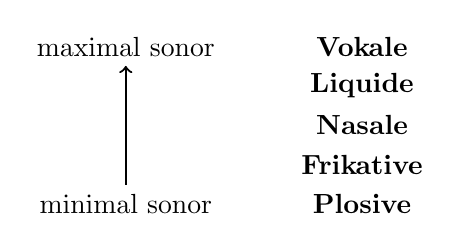
\begin{tikzpicture}
    \node (min)                             {minimal sonor};
    \node (plo) at ([shift={( 3,0)}]   min) {\textbf{Plosive}};
    \node (fri) at ([shift={( 0,0.5)}] plo) {\textbf{Frikative}};
    \node (nas) at ([shift={( 0,0.5)}] fri) {\textbf{Nasale}};
    \node (liq) at ([shift={( 0,0.5)}] nas) {\textbf{Liquide}};
    \node (vok) at ([shift={( 0,0.5)}] liq) {\textbf{Vokale}};
    \node (max) at ([shift={(-3,0)}]   vok) {maximal sonor};
    \draw [->, thick] (min) to (max);
  \end{tikzpicture}
  \caption{Sonoritätshierarchie}
  \label{fig:sonoritaet085}
\end{figure}

\begin{figure}[!htbp]
  \centering
  \begin{tikzpicture}
    \node (P1) at (0, 0.0) {P};
    \node (F1) at (1, 0.5) {F};
    \node (N1) at (2, 1.0) {N};
    \node (L1) at (3, 1.5) {L};
    \node (V0) at (4, 2.0) {V};
    \node (L2) at (5, 1.5) {L};
    \node (N2) at (6, 1.0) {N};
    \node (F2) at (7, 0.5) {F};
    \node (P2) at (8, 0.0) {P};
    \draw [->] (P1) to (F1);
    \draw [->] (F1) to (N1);
    \draw [->] (N1) to (L1);
    \draw [->] (L1) to (V0);
    \draw [->] (V0) to (L2);
    \draw [->] (L2) to (N2);
    \draw [->] (N2) to (F2);
    \draw [->] (F2) to (P2);
  \end{tikzpicture}
  \caption{Sonorität für die Segmentklassen in der schematischen Silbe}
  \label{fig:sonoritaet086}
\end{figure}

Das \textit{Sonoritätsprinzip} (oder \textit{Prinzip der Silbenkontur}) besagt, dass die Segmente in Silben der Sonoritätskontur folgen müssen, und Silben wie *[ʁka] (LPV), *[ɔpm] (VPN) oder *[lkl] (LPL) sind damit ausgeschlossen.

\paragraph*{Kern}

Man kann das Sonoritätsprinzip auch anders formulieren, indem man zunächst feststellt, dass jede Silbe einen Vokal enthält, der ihren \textit{Kern} bildet.%
\footnote{Dies stimmt für den deutschen Standard, wie er hier beschrieben wurde.
In anderen Varietäten und anderen Beschreibungen des Standards können auch silbische Liquide und Nasale im Silbenkern stehen.
In einigen anderen Sprachen können ganz unterschiedliche Typen von Segmenten Silbenkerne bilden.}
Vokale sind wie erwähnt die sonsorsten Segmente.
Vor diesem vokalischen Kern stehen Konsonanten mit nach außen fallender Sonorität im sogenannten \textit{Anfangsrand}.
Nach dem Kern stehen ggf.\ ebenfalls mit nach außen fallender Sonorität Konsonanten im sogenannten \textit{Endrand}.
Kern und Endrand bilden zusammen den sogenannten \textit{Reim} der Silbe.
Silben mit nicht gefülltem Endrand heißen \textit{geschlossen}, solche mit gefülltem Endrand \textit{offen}.

Mit der eingeführten Terminologie können wir die Struktur einer Silbe beschreiben, unter anderem in Baumform.
Beispiele dafür werden in \ref{fig:silbenstruktur040a} und \ref{fig:silbenstruktur040b} gezeigt.

\begin{figure}[!htbp]
  \centering
  \centering
  \begin{forest}
    [Silve, calign=last
      [Anfangsrand, ake
        [v]
      ]
      [Reim
        [Kern, ake
          [oː]
        ]
      ]
    ]
  \end{forest}
  \caption{Beispiel für Silbenstruktur (\textit{wo})}
  \label{fig:silbenstruktur040a}
\end{figure}

\begin{figure}[!htbp]
  \centering
  \begin{forest}
    [Silbe, calign=last
      [Anfangsrand, ake, calign=first
        [f][ʁ]
      ]
      [Reim, calign=first
        [Kern,ake
          [ɛ]
        ]
        [Endrand, ake, calign=last
          [m][t]
        ]
      ]
    ]
  \end{forest}
  \caption{Beispiel für Silbenstruktur (\textit{fremd})}
  \label{fig:silbenstruktur040b}
\end{figure}

Das Prinzip des Silbenkerns besagt, dass jede Silbe einen Kern haben muss, der im deutschen Standard ein Vokal (ggf.\ ein silbischer Nasal oder Liquid) sein muss.
Es spielt zunächst keine Rolle, ob der Kern mit einem kurzen Vokal, einem langen Vokal oder einem Diphthong gefüllt ist.

\paragraph*{Präferierte Ränder}

Da im Kern ein genau Vokal stehen muss, aber in den Rändern unter Umständen mehrere Konsonanten stehen, sind insbesondere die in einer Sprache möglichen Abfolge der Konsonanten in den Rändern interessant.
Neben der Bedingung, dass stets die Sonoritätskontur eingehalten werden muss, gelten einzelsprachlich (hier also für das Deutsche) bestimmte Präferenzen.
Wir beschreiben diese Präferenzen hier gleich unter Ausschluss der extrasilbischen Segmente (siehe unten).

Im Wesentlichen ist im deutschen Kernwortschatz ein Anfangsrand, der aus zwei Segmenten besteht, mit einem äußeren Plosiv oder Frikativ gefolgt von einem Liquid besetzt.
Typisch sind also Silben (hier Einsilbler, also einsilbige Wörter) wie \textit{treu} /trʁɔ͡ʏ/ [tʁɔ͡ʏ], \textit{kräh} /kʁɛ/ [kʁɛː], \textit{Bräu} /bʁɔ͡ʏ/ [bʁɔ͡ʏ], \textit{frei} /fʁa͡ɛ/ [fʁa͡ɛ], \textit{Klee} /kle/ [kleː], \textit{blau} /bla͡ɔ/ [bla͡ɔ], \textit{flieh} /fli/ [fliː].
Daneben gibt es seltener die Kombination [kv] wie in \textit{Qual} /kval/ [kvaːl] und [kn] wie in \textit{Knie} /kni/ [kniː] oder der Erstsilbe von \textit{Knabe} /knabə/ [knaːbə].
Mit Ausnahme der extrasilbischen [ʃ] wie in \textit{Sprung} /ʃpʁʊng/ [ʃpʁʊŋ] ist damit der Anfangsrand beschrieben.

Der Endrand, der aus zwei Segmenten besteht, hat im Deutschen wesentlich mehr Besetzungsmöglichkeiten als der Anfangsrand.
Sonoritätsplateaus kommen nur mit Konsonanten -- und in nicht flektierten Simplizia sehr selten -- vor wie in \textit{Abt} /apt/ [ʔapt].
Bereits etwas häufiger (im Sinne der Typenhäufigkeit) sind Kombinationen aus Frikativ und Plosiv wie in \textit{Schaft} /ʃăft/ [ʃaft] oder \textit{Ast} /ăst/ [ʔast].
Kombinationen aus Nasal und Frikativ wie in \textit{Ramsch} /ʁămʃ/ [ʁamʃ] oder Hanf /hănf/ [hanf] kommen vor, sind aber nicht sonderlich häufig.
Solche aus Nasal und Plosiv sind präferiert homorgan (also am selben Artikulationsort gebildet, siehe \textit{rund} /ʁʊnd/ [ʁʊnt], \textit{Bank} /bănk/ [bank] und \textit{Klump} /klʊmp/ [klʊmp].
Es gibt allerdings auch (in Simplizia) selten [mt] wie in \textit{Amt} /ămt/ [ʔamt].
Ganz typisch und typenhäufig sind dann die Endränder, die spiegelbildlich zum Anfangsrand aus einem Liquid gefolgt von einem Plosiv oder Frikativ bestehen.
Beispiele sind \textit{Bart} /băʁt/ [ba͡ət], \textit{kalt} /kălt/ [kalt], \textit{Berg} /bɛ̆ʁg/ [bɛ͡ək], \textit{welk} /vɛ̆lk/ [vɛlk], \textit{Barsch} /băʁʃ/ [ba͡əʃ], \textit{falsch} /fălʃ/ [falʃ], \textit{Torf} /tɔʁf/ [tɔ͡əf]. 
Im Gegensatz zum Anfangsrand gibt es allerdings auch -- wiederum seltene -- Kombinationen aus Liquid und Nasal wie in \textit{Qualm} /kvălm/ [kvalm] oder \textit{Harn} /hăʁn/ [ha͡ən].

Es sind also nicht alle beliebigen Kombinationen aus Segementen in den Rändern denkbar, und der Prototyp des duplexen Randes ist der aus einem äußerem Plosiv oder Frikativ und einem inneren Liquid.

\paragraph*{Silbengewicht}

Der Silbenreim (also die Konstituente aus Kern und Endrand) spielt an verschiedenen Stellen im System eine Rolle.
Unter anderem ist der Reim relevant für die Bestimmung möglicher Silbentypen, wenn man die Einheit der \textit{More} -- die Einheit des \textit{Silbengewichts} -- hinzunimmt.
Damit kann die Komplexität des Silbenreims insgesamt beschrieben werden.
Kurze Vokale im Kern zählen eine More, lange Vokale und Diphthonge zählen zwei Moren.
Man sieht also, dass das Gewicht der Silbe durchaus etwas mit Länge zu tun hat.
Allerdings zählen wir jeden Konsonanten im Endrand ebenfalls mit einer More, und das Konzept der Länge ist für Konsonanten zunächst einmal nicht definiert, weswegen man auf den Begriff des Gewichts ausweicht.
Nur der Reim zählt zum Silbengewicht, der Anfangsrand ist völlig irrelevant.

Wir finden im Deutschen ein- bis dreimorige Silben.
Zunächst wird der Kernwortschatz beschrieben.
Einmorig sind im Kernwortschatz nur offene Schwa-Silben und unbetonte Silben mit ungespanntem Vokal (vor allem [ɪ]).%
\footnote{Bis zur dritten Auflage wurden in EGBD die unbetonten offenen Silben mit ungespanntem Vokal nicht beschrieben.}
Solche Schwa-Silben sind sehr häufig, zum Beispiel die Zweitsilben in \textit{Tüte} /tytə/ [ˈtyː.tə], \textit{Sahne} /zanə/ [ˈzaː.nə], \textit{Stühle} /ʃtylə/ [ˈʃtyː.lə] usw.
Die unbetonten offenen Silben mit ungespanntem Vokal kommen vor allem in drei- oder mehrsilbigen derivierten und\slash oder flektierten Wortformen vor, zum Beispiel \textit{wenigere} /venɪgəʁə/ [ˈveː.nɪ.gə.ʁə] (Silbe [nɪ]), \textit{schwächliche} /ʃvɛ̆çlɪçə/ [ˈʃvɛç.lɪ.çə] (Silbe [lɪ]), aber auch in derivierten Wörtern wie \textit{Neunziger} /nɔ͡ʏnt͡sɪgəʁ/ [nɔ͡ʏn.t͡sɪ.gɐ] (Silbe [t͡sɪ]).%
\footnote{In den Wörtern mit ungespanntem Vokal kein kein Silbengelenk vorliegen, weil dies nur im Trochäus auftritt.
Die Silbifizierung *[ˈnɔ͡ʏn.t͡sɪg̣ɐ] wäre also inkorrekt.
Das Movierungssuffix \textit{-in} hat immer einen Nebenakzent, und in den entsprechenden Silben liegt daher ein Silbengelenk vor, also \textit{Schülerinnen} /ʃyləʁɪnən/ [ˈʃyː.lə.ˌʁɪṇən].}
Da dieser Silbentypus nicht betont sein kann, gibt es auch keine Einsilbler, die aus solchen Silben bestehen.

Zweimorig sind (ob betont oder unbetont) entweder (1) offene Silben mit langem Vokal oder mit Diphthong oder (2) geschlossene Silben mit kurzem Vokal und einfach besetztem Endrand.
Den ersten Fall illustrieren (im Einsilbler) \textit{nah} /na/ [naː], \textit{Vieh} /fi/ [fiː] und \textit{schlau} /ʃla͡ɔ/ [ʃla͡ɔ], den zweiten \textit{schlapp} /ʃlăp/ [ʃlap], \textit{Napf} /năp͡f/ [nap͡f] und \textit{Bann} /băn/ [ban].%
\footnote{In \textit{Napf} ist [p͡f] eine Affrikate und zählt daher einmorig.}

Als dreimorige Silben kommen (wiederum betont der unbetont) Silben mit kurzem Vokal und doppelt gefülltem Endrand oder Silben mit langem Vokal (bzw.\ Diphthong) und einfach gefülltem Endrand in Frage.
Den ersten Fall bebeispielen die Einsilbler \textit{Schwank} /ʃvănk/ [ʃvaŋk], \textit{Kalb} /kălb/ [kalp] und \textit{Korb} /kɔʁb/ [kɔ͡əp], den zweiten \textit{Mus} /muz/ [muːs], \textit{lieb} /lib/ [liːp] und \textit{Hag} /hag/ [haːk].

Es gibt im Deutschen also gemäß dem Prinzip der Silbenschwere nur unbetonte einmorige Silben, außerdem zweimorige und dreimorige Silben (betont oder unbetont).
Betonte einmorige Silben wären \textit{überleicht}, vier- oder mehrmorige Silben \textit{überschwer}.
Wie Wörter wie \textit{Herbsts} /hɛ̆ʁbztz/ [hɛ͡əpsts], das scheinbar sechsmorig zu sein scheint -- in dieses Bild passen, wird im nächsten Absatz geklärt.

\paragraph*{Extrasilbizität}

\paragraph*{Anfangsrandmaximierung}

\paragraph*{Anfangsrand-Füllung}

\paragraph*{Silbengelenkbildung}



\section{Analysen zur Fuß- und Wortphonologie}
\label{sec:phonologie:analysenzurfussundwortphonologie}

\subsection{Prinzipien der Fuß- und Wortphonologie}

\paragraph*{Akzent und Nebenakzent}

\paragraph*{Stammbetonung, phonologisches Wort, prosodisches Wort}

\paragraph*{Komposita}

\paragraph*{Affixe und Akzent}

\paragraph*{Fußbildung}




